\documentclass[../main.tex]{subfiles}

% ======================== Preamble ================================================%
\setcounter{table}{0}
\setcounter{figure}{0}
% ======================== Document: Appendix C: Province-month panels ======================== %

\begin{document}
\section{Appendix: Province-month panel results}
\label{sec:appendixc}

\setcounter{table}{0}
\setcounter{figure}{0}
\begin{table}[htbp!]
    \centering
    \begin{threeparttable}
    \caption{DD specifications for monthly patent applications}
        \label{tab:dd_twfe_patents_monthly}
        
\begin{tabular}[t]{lccc}
\toprule
  & (1) & (2) & (3)\\
\midrule
Treatment x Post & \num{-0.058} & \num{0.088} & \num{0.077}\\
\textbf{} & \textbf{(\num{0.042})} & \textbf{(\num{0.070})} & \textbf{(\num{0.083})}\\
\midrule
Explained variable &  & $\ln(\text{Patents}+1)$ & \\
$N$ & \num{1968} & \num{1968} & \num{1968}\\
Adj. $R^2$ & \num{0.942} & \num{0.952} & \num{0.952}\\
Adj. within $R^2$ & \num{0.000} & \num{0.168} & \num{0.177}\\
RMSE & \num{0.314} & \num{0.285} & \num{0.283}\\
\bottomrule
\end{tabular}
}
        \begin{tablenotes}
            \small
            \item \textit{Notes}: Clustered standard errors at the province and monthly level shown in parentheses. Specifications include fixed effects for provinces and months and controls for their quarterly counterpart in Table \ref{tab:dd_twfe_patents}. ***$p<0.01$, **$p<0.05$, *$p<0.1$.
        \end{tablenotes}
    \end{threeparttable}
\end{table}

\begin{table}[htbp!]
    \centering
    \begin{threeparttable}
    \label{tab:dd_twfe_patents_by_section_monthly}
    \caption{Difference-in-differences results for monthly patent applications by IPC section}
    
\begin{tabular}[t]{lcccccccc}
\toprule
  & (1) & (2) & (3) & (4) & (5) & (6) & (7) & (8)\\
\midrule
Treatment x Post & \num{0.319}*** & \num{0.346}** & \num{0.000} & \num{0.099}* & \num{-0.452}*** & \num{0.229}** & \num{-0.151} & \num{0.193}\\
\textbf{} & \textbf{(\num{0.071})} & \textbf{(\num{0.124})} & \textbf{(\num{0.125})} & \textbf{(\num{0.048})} & \textbf{(\num{0.060})} & \textbf{(\num{0.096})} & \textbf{(\num{0.101})} & \textbf{(\num{0.108})}\\
\midrule
Patent section (IPC) & A & B & C & D & E & F & G & H\\
$N$ & \num{1968} & \num{1968} & \num{1968} & \num{1968} & \num{1968} & \num{1968} & \num{1968} & \num{1968}\\
Adj. $R^2$ & \num{0.823} & \num{0.853} & \num{0.767} & \num{0.163} & \num{0.849} & \num{0.774} & \num{0.877} & \num{0.860}\\
Adj. within $R^2$ & \num{0.049} & \num{0.038} & \num{0.051} & \num{0.016} & \num{0.054} & \num{0.014} & \num{0.044} & \num{0.057}\\
RMSE & \num{0.414} & \num{0.396} & \num{0.395} & \num{0.248} & \num{0.380} & \num{0.405} & \num{0.375} & \num{0.393}\\
\bottomrule
\end{tabular}
}
    \begin{tablenotes}
        \footnotesize
        \item \textit{Notes}: All specifications include controls in Specification (3) of Table \ref{tab:dd_twfe_patents_monthly}, not shown for brevity and fixed effects for provinces and months. Clustered standard errors at the province and month level are shown in parentheses. 
        \item  Sections of the IPC are A: Human Necessities, B: Performing Operations; Transporting, C: Chemistry; Metallurgy, D: Textiles; Paper, E: Fixed Constructions, F: Mechanical Engineering; G: Physics, H: Electricity. Patents with multiple sections are not included. ***$p<0.01$, **$p<0.05$, *$p<0.1$.
    \end{tablenotes}
    \end{threeparttable}
\end{table}

\begin{landscape}
\begin{figure}[htbp!]
        \centering
        \caption{Event study plot for monthly patent applications}
        \label{fig:event_study_patents_monthly}
        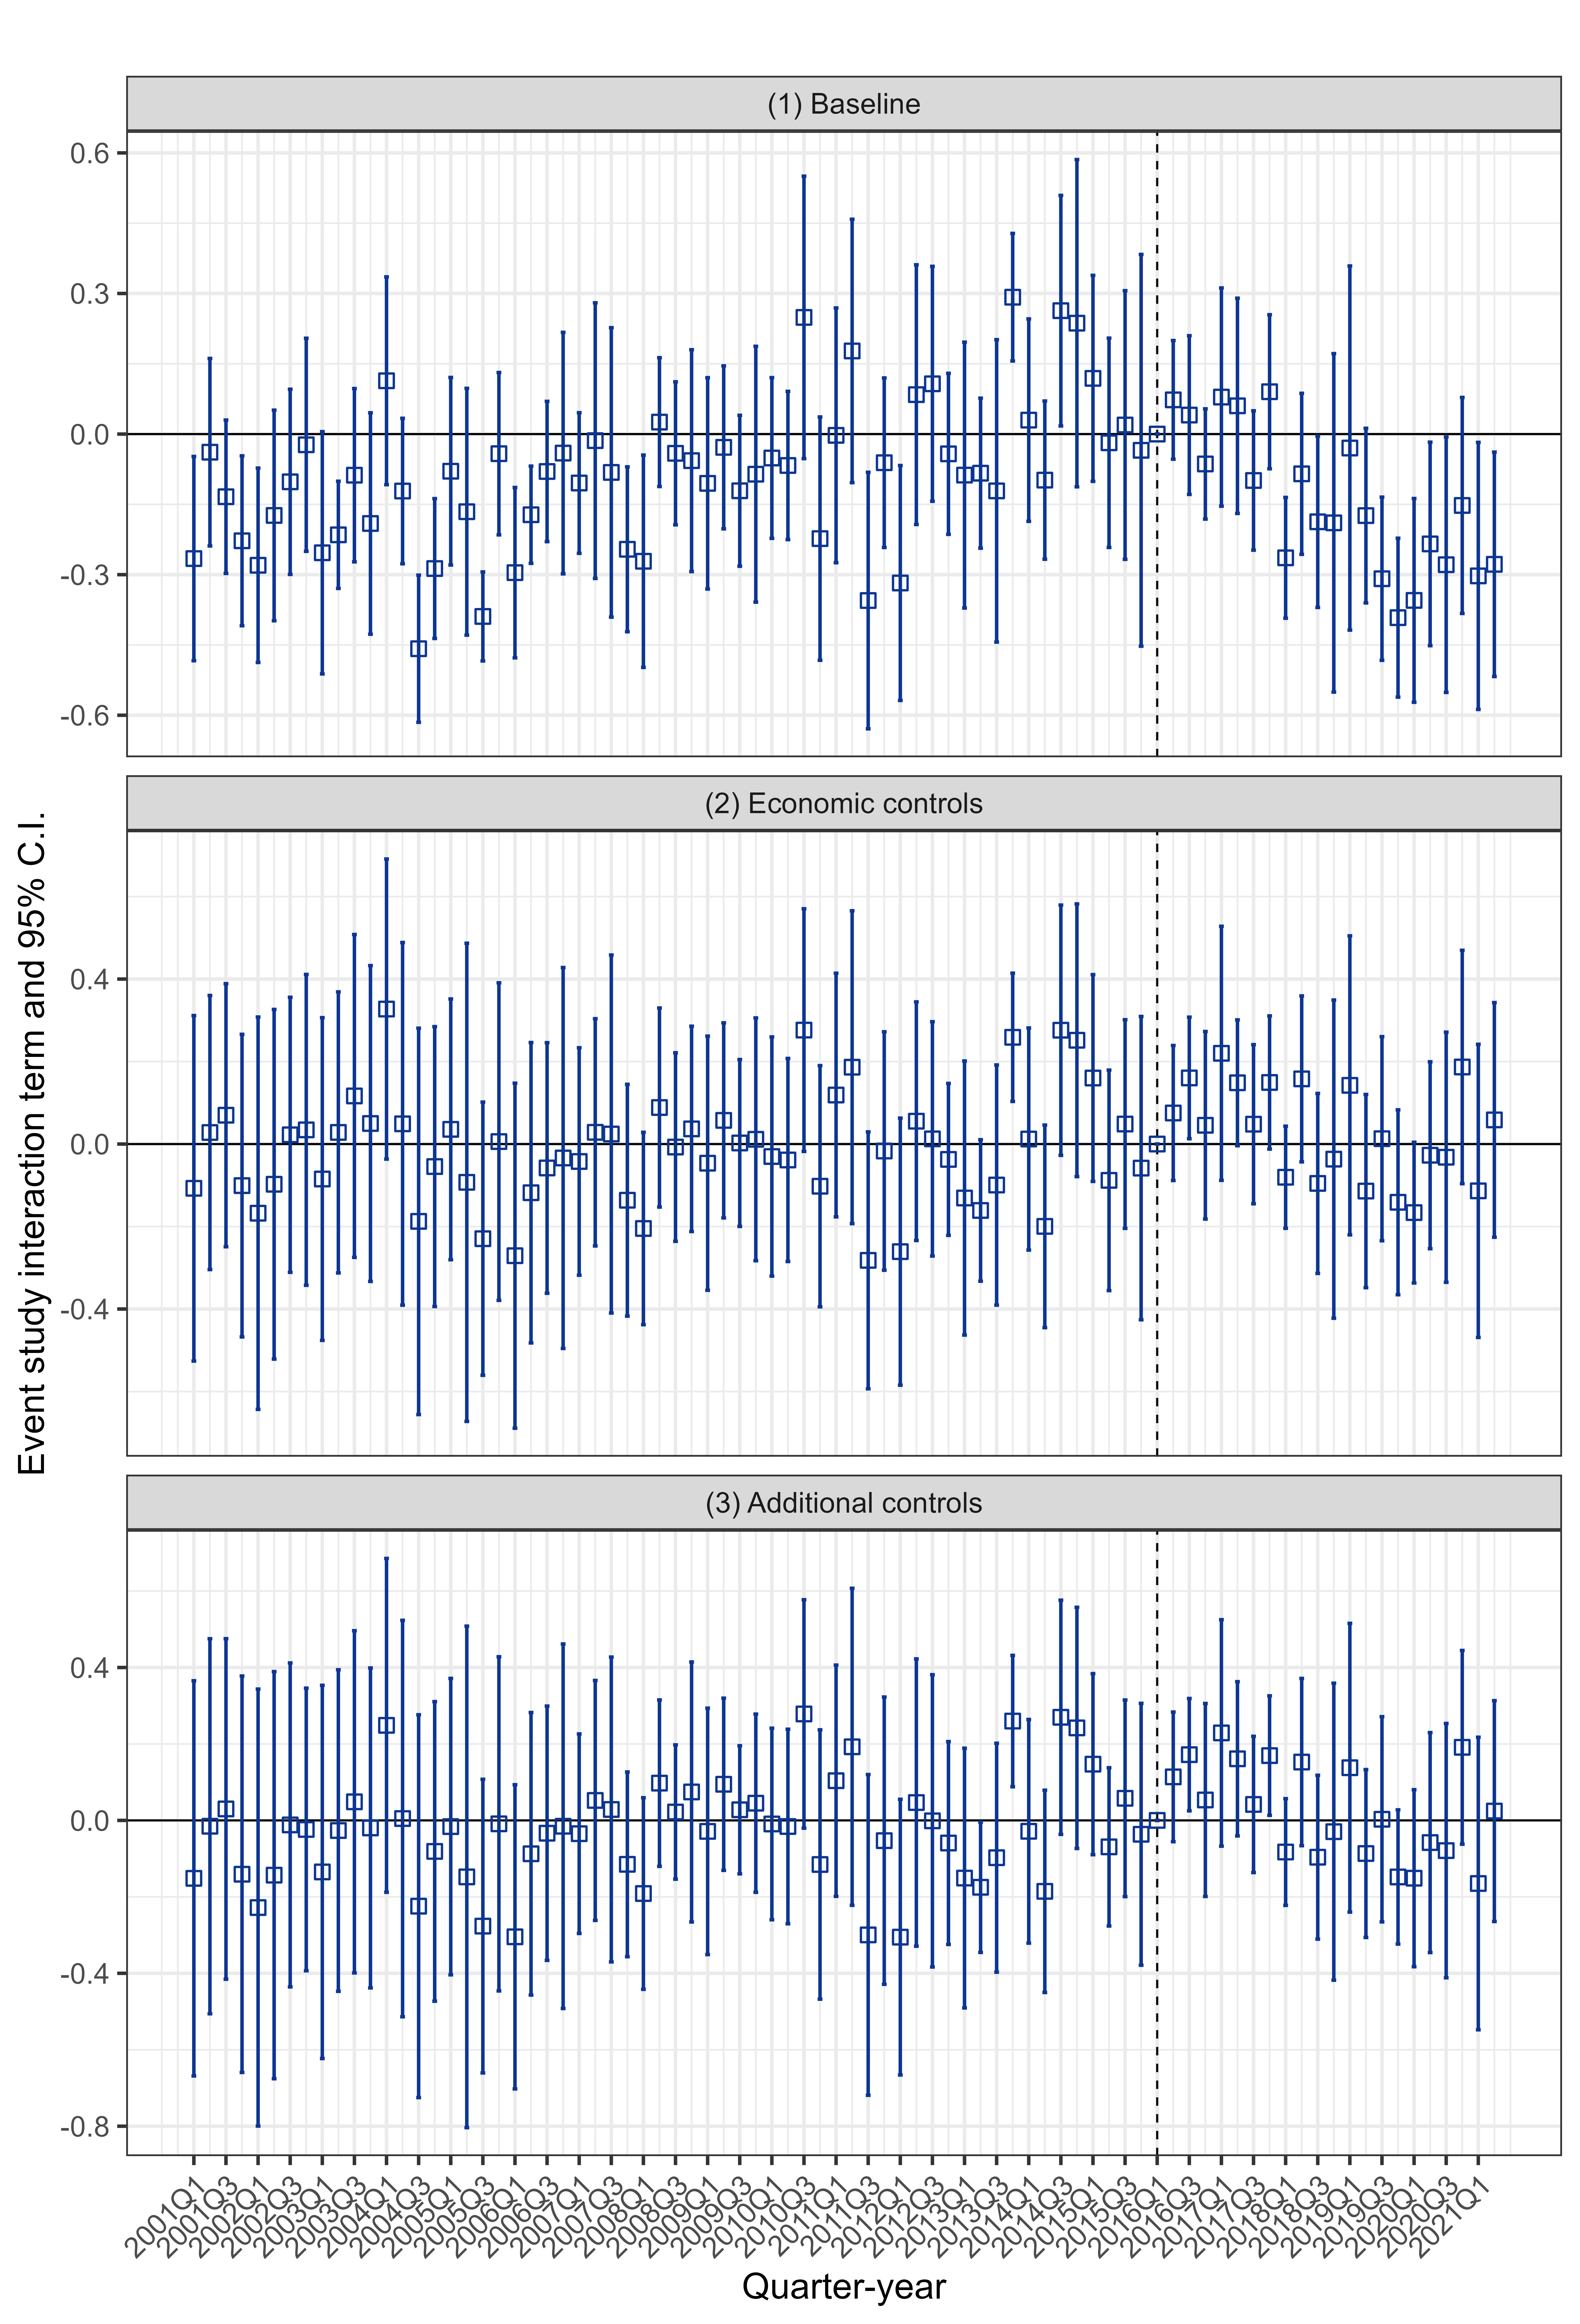
\includegraphics{\subfix{../../figures/event-studies/monthly/patents_faceted.png}}
        \begin{minipage}{0.9\textwidth}
            \footnotesize
            \textit{Notes}: The figure shows the estimated coefficients of the interaction term between period and treatment binary variables in Equation \ref{eq:event_study} for each month. The points represent the point estimate, while the error bars represent the 95\% confidence cluster-robust interval. The vertical line represents the start of the AITC intervention in January 2017, with the reference level being the month before the intervention. Baseline, economic, and additional controls specifications include the controls seen in specifications (1) through (3) in Table \ref{tab:dd_twfe_patents_monthly}. 
        \end{minipage}
    \end{figure}
\begin{figure}[htbp!]
        \centering
        \caption{Event study plot for monthly patent applications by IPC section}
        \label{fig:event_study_patents_section_monthly}
        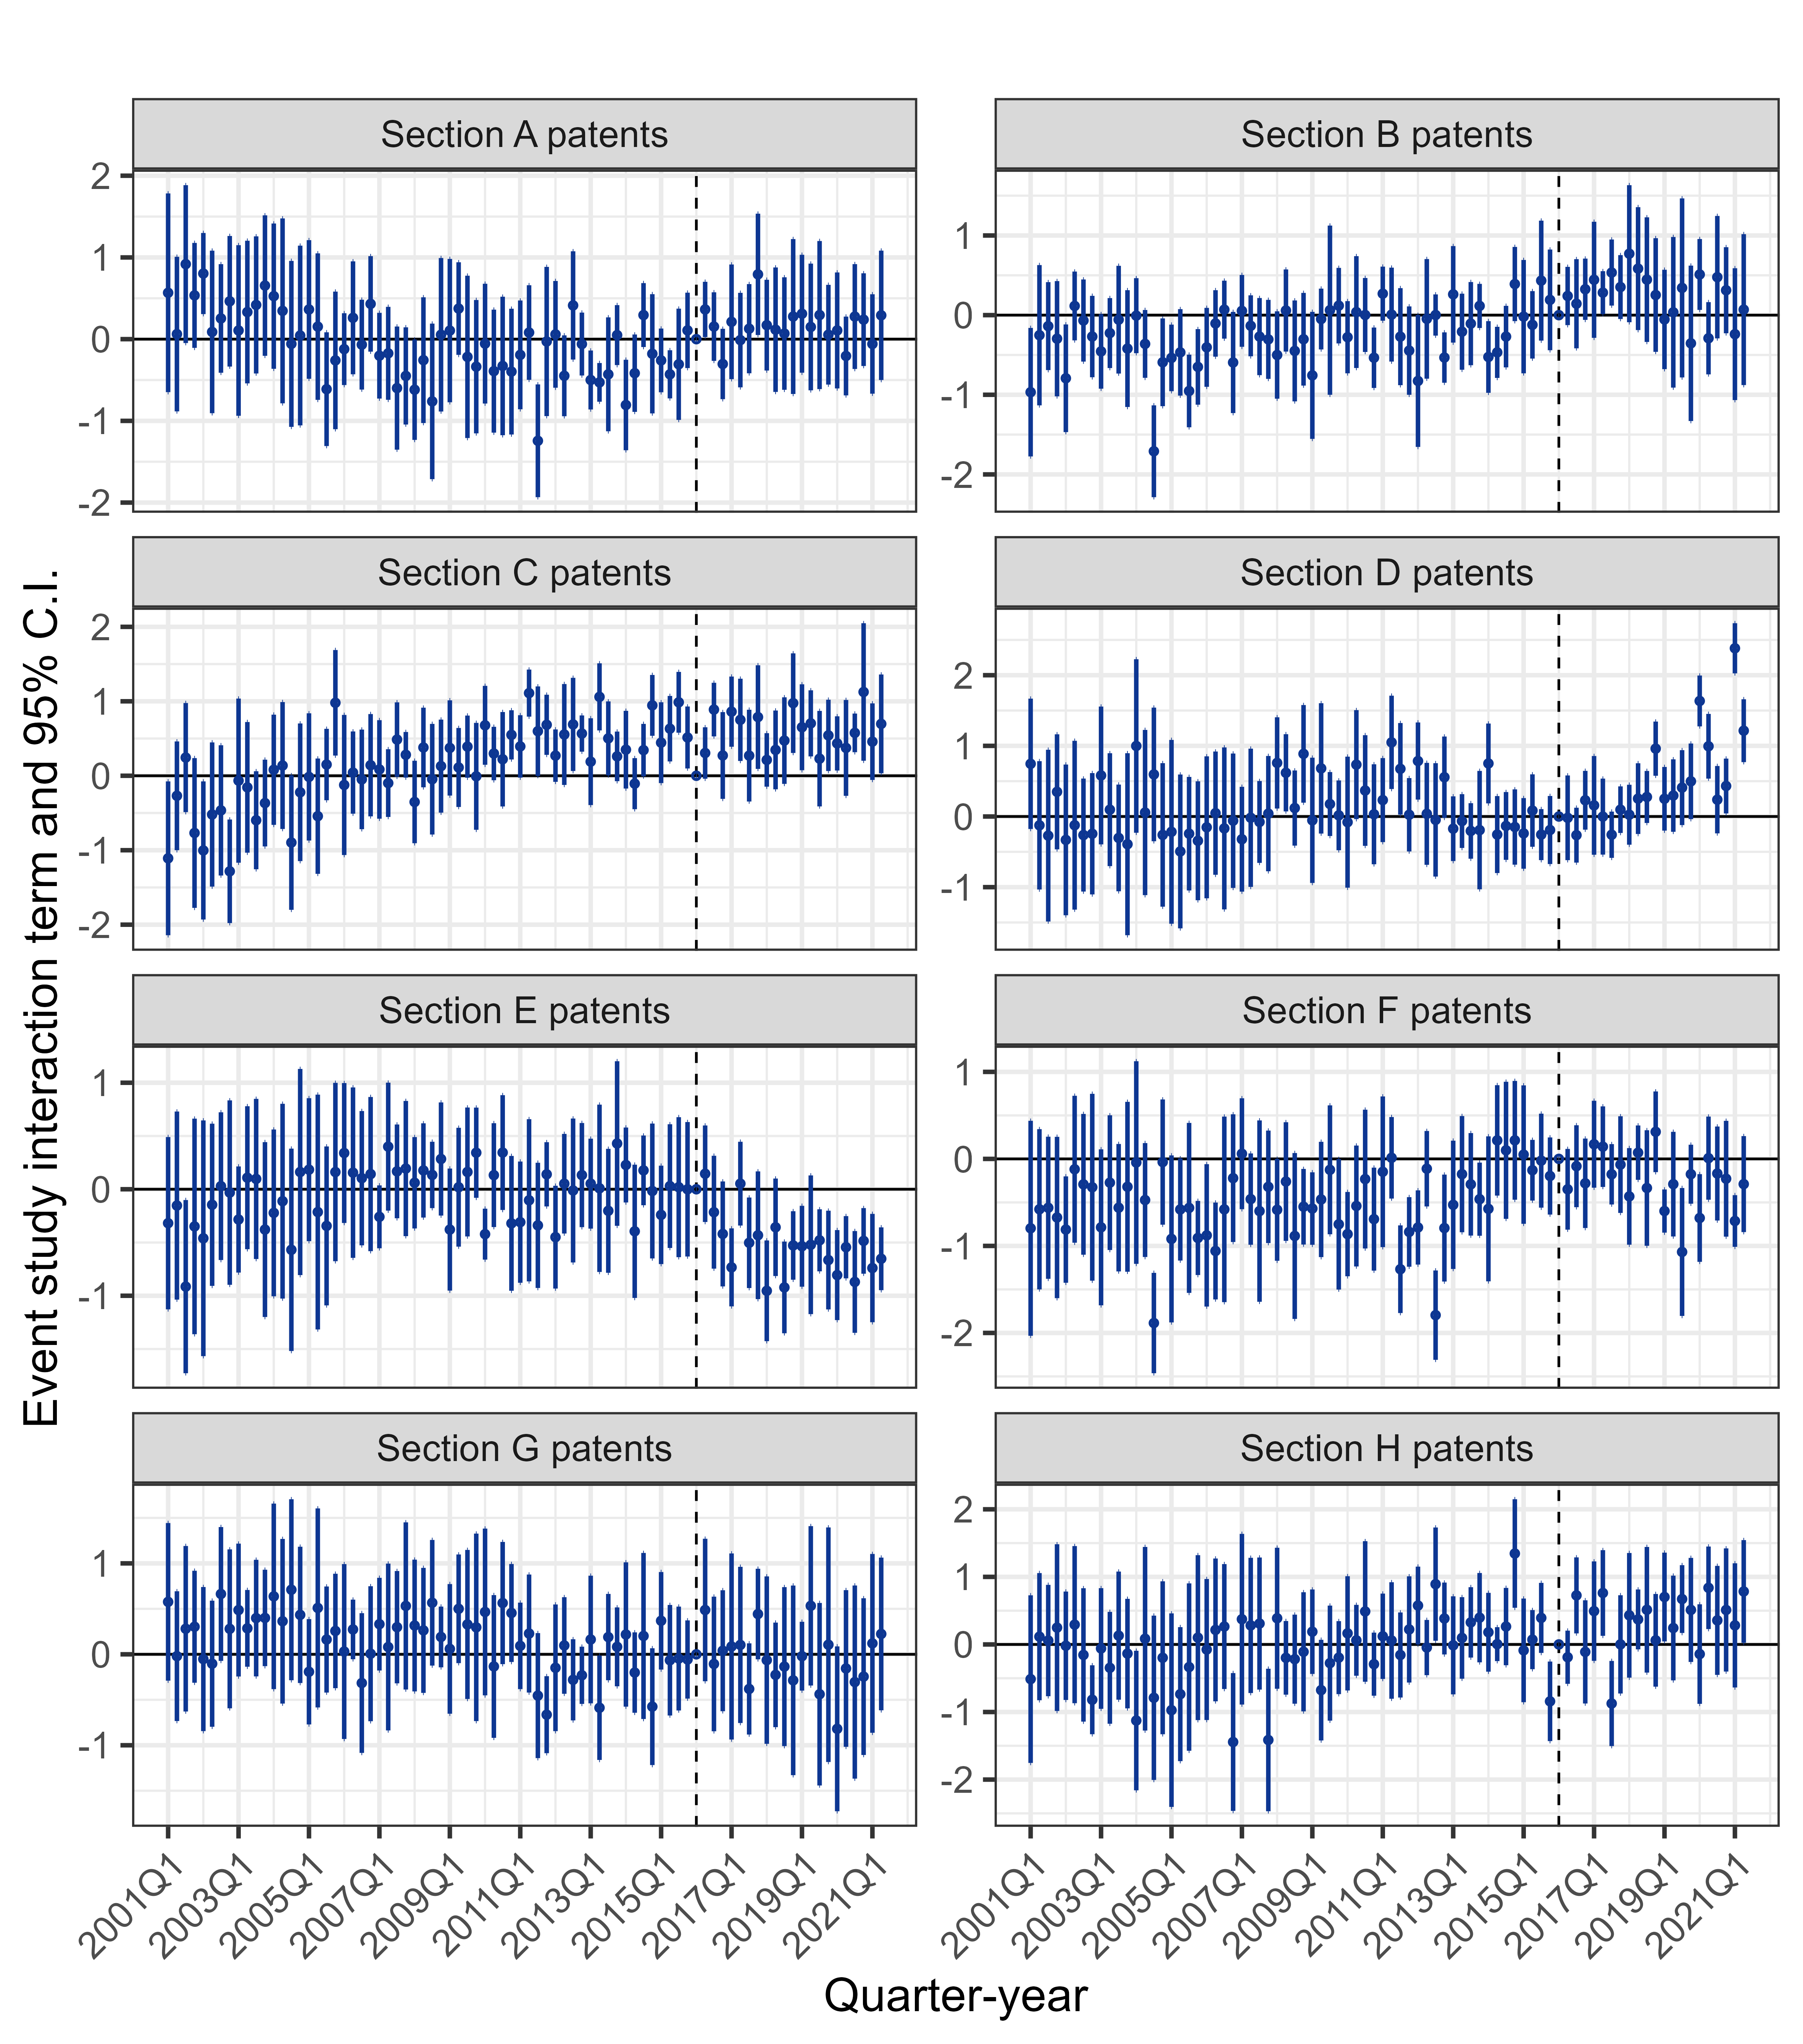
\includegraphics{\subfix{../../figures/event-studies/monthly/patent_sections_faceted.png}}
        \begin{minipage}{0.9\textwidth}
            \footnotesize
            \textit{Notes}: The figure shows the estimated coefficients of the interaction term between period and treatment binary variables in Equation \ref{eq:event_study} for each month, separated by IPC section. The lines represent point estimates, while the shaded areas represent the 95\% confidence cluster-robust intervals. The vertical line represents the start of the AITC intervention in January 2017, with the reference level being the quarter before the intervention. Controls are the same as those in Specification (3) in Table \ref{tab:dd_twfe_patents}. 
        \end{minipage}
    \end{figure}
\end{landscape}


\end{document}
